% TODO:
% - 

%%%%%%%%%%%%%%%%%%%%%%%%%%%%%%%%%%%%%%%%%%%%%%%%%%%%
% documentclss
\documentclass[]{beamer}
%\documentclass[handout]{beamer} %Drucker Version


%%%%%%%%%%%%%%%%%%%%%%%%%%%%%%%%%%%%%%%%%%%%%%%%%%%%
% packages

\usepackage[utf8]{inputenc}
\usepackage[ngerman]{babel}
\usepackage[T1]{fontenc}

\usepackage{setspace}
\usepackage{microtype}
\usepackage{lmodern}

\usepackage{graphicx}
\graphicspath{{images/}}

\hypersetup{
  pdftex,
  bookmarks, bookmarksopen, bookmarksopenlevel=1, bookmarksnumbered=true,
  pdfpagemode={UseNone},
  pdfpagelayout={SinglePage},
  plainpages=false,
  pdfkeywords={Systemdesk},
  pdfsubject={Systemdesk},
  pdftitle={Systemdesk},
  pdfauthor={Martin Wichmann}
}

\usepackage{booktabs}
\usepackage{multirow}


\newtranslation[to=ngerman]{Example}{Beispiel}


\usetheme{Warsaw}



%\AtBeginSection[]
%{
%   \begin{frame}
%        \frametitle{Inhaltsübersicht}
%        \tableofcontents[currentsection,currentsubsection]
%   \end{frame}
%}



%%%%%%%%%%%%%%%%%%%%%%%%%%%%%%%%%%%%%%%%%%%%%%%%%%%%
% Title
\author{Martin Wichmann}
\title{Einführung Systemdesk}
\date{\today}
\institute{Ostfalia Hochschule für angewandte Wissenschaften}




%%%%%%%%%%%%%%%%%%%%%%%%%%%%%%%%%%%%%%%%%%%%%%%%%%%%
% begin document
\begin{document}

\begin{frame}
\maketitle
\end{frame}


\begin{frame}
\frametitle{Inhaltsübersicht}
\tableofcontents
\end{frame}





%%%%%%%%%%%%%%%%%%%%%%%%%%%%%%%%%%%%%%%%%%%%%%%%%%%%%%%%%%%%%%%%%%%5
% Einleitung
\section{Einleitung}
\label{sec:einleitung}

\begin{frame}
\frametitle{Einleitung}
    \begin{itemize}
    \item SystemDesk 3.1
    \item Verwendungzweck:
        \begin{itemize}
        \item Autosar Systemmodelling
        \item Behavior Modelling (teilweise)
        \item ECU Config und RTE Generierung (teilweise)
        \end{itemize}
    \item Einführung nur grober Überblick. Genauere Infos:
        \begin{itemize}
        \item SystemDesk Tutorial (vor allem Kapitel 2-4)
        \item SystemDesk Handbuch
        \end{itemize}
    \end{itemize}
\end{frame}


\begin{frame}
\frametitle{Programm Aufbau I}
    \begin{figure}
       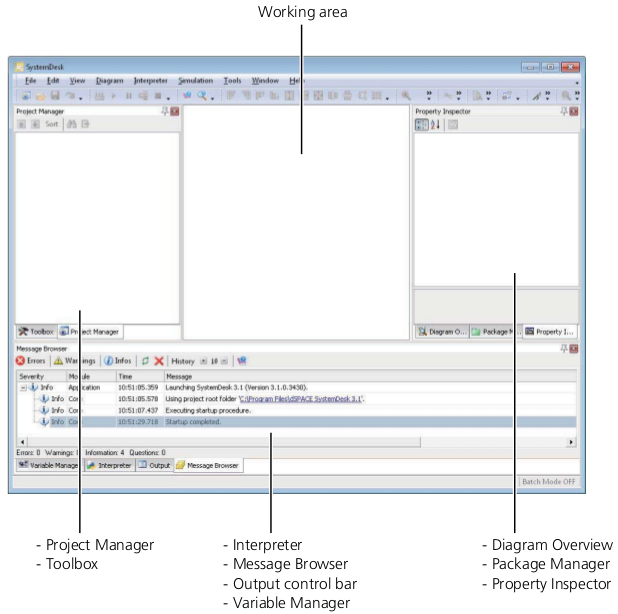
\includegraphics[width=7.5cm]{programm}
    \end{figure}
\end{frame}

\begin{frame}
\frametitle{Programm Aufbau II}
    \begin{figure}
       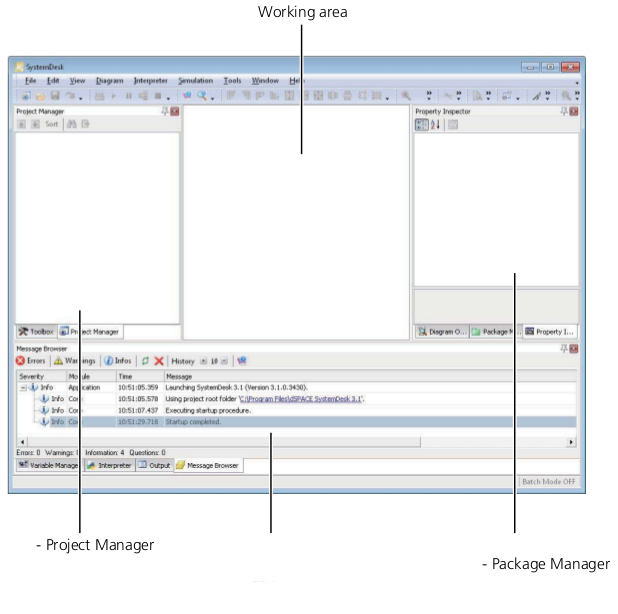
\includegraphics[width=7.5cm]{programm_clean}
    \end{figure}
\end{frame}


\begin{frame}
\frametitle{Programm Aufbau III}
    \begin{itemize}
    \item Project Manager
    \begin{itemize}
        \item Project Library
        \item Systeme
    \end{itemize}
    \item Package Manager
    \begin{itemize}
        \item Nötig für Autosar Export
    \end{itemize}
    \item Working Area
    \begin{itemize}
        \item Darstellung von Diagrammen
    \end{itemize}
    \item Interpreter
    \begin{itemize}
        \item Python Zugriff über COM
    \end{itemize}
    \end{itemize}
\end{frame}




\begin{frame}
\frametitle{Beispiel}
    \begin{figure}
       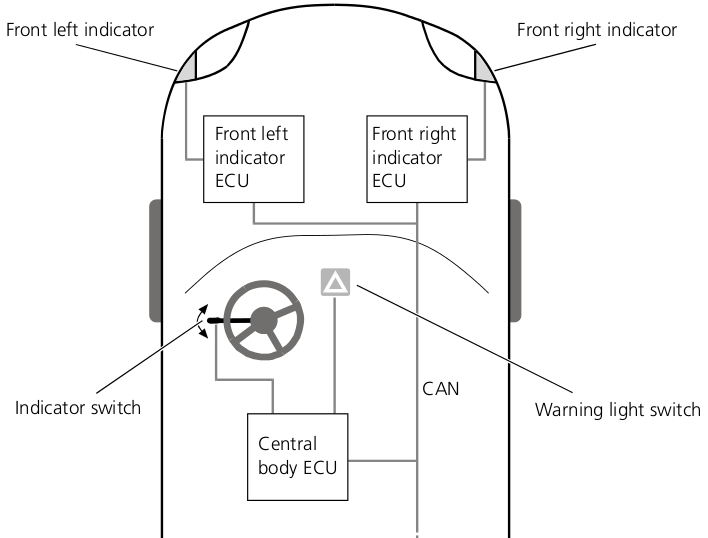
\includegraphics[width=8.5cm]{beispiel}
    \end{figure}
\end{frame}



%%%%%%%%%%%%%%%%%%%%%%%%%%%%%%%%%%%%%%%%%%%%%%%%%%%%%%%%%%%%%%%%%%%5
% Arbeitsprinzipien
\section{Arbeitsprinzipien}
\label{sec:arbeitsprinzipien}

\begin{frame}
\frametitle{Arbeitsprinzipien - Project Library}
    \begin{itemize}
    \item Design aller Elemente
    \item Verknüpfungen
    \begin{itemize}
        \item Datatyp -> Variable
        \item SWC -> Composition
    \end{itemize}
    \item Diagramme getrennt von Model
    \end{itemize}
\end{frame}



\begin{frame}
\frametitle{Arbeitsprinzipien - System}
    \begin{itemize}
    \item ”Implementierung” der Project Library
    \item Software Architecture
        \begin{itemize}
            \item Top Level Composition
            \item Verknüpfungen zu SWCs und Compositionen
        \end{itemize}
    \item Hardware Topology
        \begin{itemize}
            \item ECUs
        \end{itemize}
    \item Network Communication
    \end{itemize}

\end{frame}



%%%%%%%%%%%%%%%%%%%%%%%%%%%%%%%%%%%%%%%%%%%%%%%%%%%%%%%%%%%%%%%%%%%5
% Literaturangaben
\appendix
\section*{Literatur}
\label{sec:Literatur}

\begin{frame}
\begin{thebibliography}{10}

\bibitem[1]{1} \textsc{dSpace}: {\em SystemDesk Tutorial.} dSpace, 2011.

\end{thebibliography}
\end{frame}





















\end{document}










